\documentclass[11pt]{article}
\usepackage{mathblatt}
% Selbstlernfassung
% Gesetzt aus aufgaben.jsonl (Prüfstein Musterauftrag, 09.10.2026).
\usepackage{enumitem}
\usetikzlibrary{calc}
\newgeometry{a4paper,margin=18mm,top=15mm,bottom=20mm,footskip=9mm}
\pagestyle{fancy}\fancyhf{}\renewcommand{\headrulewidth}{0pt}
\fancyfoot[L]{\footnotesize\color{mbgrau}Satz des Pythagoras: die Hypotenuse berechnen}
\fancyfoot[R]{\footnotesize\color{mbgrau}\thepage}
\setlength{\parskip}{3pt}
\renewcommand{\kreuz}[1]{\mbox{$\square$\ #1}\quad}
\newcommand{\kreuzl}[1]{\par\hangindent1.4em\hangafter1\noindent$\square$\ #1}
\newcommand{\marke}[1]{\leavevmode\llap{\scriptsize\color{mbgrau}#1\hspace{9mm}}}
\newcommand{\aufg}[3]{\par\noindent\makebox[0pt][r]{#3}\begin{minipage}[t]{\linewidth}#1\end{minipage}\par}
\newcommand{\aufgg}[4]{\par\noindent\makebox[0pt][r]{#4}\begin{minipage}[t]{0.6\linewidth}\vspace{0pt}#1\end{minipage}\hfill
  \begin{minipage}[t]{0.37\linewidth}\vspace{0pt}\centering #2\end{minipage}\par}
\newcommand{\nr}[1]{\makebox[7mm][l]{\textbf{#1}}}
\begin{document}
\noindent{\LARGE\bfseries Satz des Pythagoras: die Hypotenuse berechnen}\par\smallskip
\noindent{\small\color{mbgrau}Selbstlernheft Klasse 9 \textperiodcentered{} mit Lösungsheft}\par\medskip
\noindent\textbf{So nutzt du das Heft:} Lies im Abschnitt das Beispiel. Rechne dann die Aufgaben der Reihe nach und vergleiche jede sofort mit dem Lösungsheft. Kreuze „kann ich“ an, wenn du die letzte Aufgabe (\emph{Ziel}) allein schaffst.\par
\noindent Mehr Aufgaben zu einem Abschnitt: Kennung deinem Nachhilfelehrer schicken (z.\,B. „mehr B“).\par\medskip
{\arrayrulecolor{mbgrau}\renewcommand{\arraystretch}{1.3}
\noindent\begin{tabular}{|>{\bfseries}p{10mm}|p{112mm}|>{\raggedleft\arraybackslash}p{10mm}|>{\centering\arraybackslash}p{14mm}|}\hline
\rowcolor{black!8} & \textbf{Abschnitt} & \textbf{Seite} & \textbf{kann ich}\\\hline
A & Hypotenuse finden und berechnen & \pageref{s:A} & $\square$\\\hline
B & Wenn die Wurzel nicht aufgeht & \pageref{s:B} & $\square$\\\hline
C & Sachaufgaben: Leiter, Rampe, Gelände & \pageref{s:C} & $\square$\\\hline
T & Probetest & \pageref{s:T} & $\square$\\\hline
\end{tabular}}\par\bigskip

\begin{tcolorbox}[colback=mbkasten,colframe=mbgrau,boxrule=0.5pt,arc=1mm,left=3mm,right=3mm,top=2mm,bottom=2mm,title={\bfseries Formel auf einen Blick},coltitle=black,colbacktitle=black!10]
\begin{minipage}[t]{0.58\linewidth}\vspace{0pt}
{\Large $c^2 = a^2 + b^2$ \qquad $c = \sqrt{a^2+b^2}$}\par\medskip
In Worten: Die Quadrate der beiden Katheten ergeben zusammen das Quadrat der Hypotenuse.\par\medskip
\textbf{So gehst du vor}\par
\nr{1}rechten Winkel suchen\par
\nr{2}gegenüber liegt die Hypotenuse (längste Seite)\par
\nr{3}$c^2 = a^2 + b^2$ ausrechnen (nicht runden)\par
\nr{4}Wurzel ziehen, am Ende runden, Einheit dazu\par\medskip
{\small Heißen die Seiten anders ($x,y,z$ oder $r,s,t$): Allein steht immer die Hypotenuse. Achtung: $c$ ist \emph{nicht} $a + b$.}
\end{minipage}\hfill
\begin{minipage}[t]{0.38\linewidth}\vspace{2mm}\centering
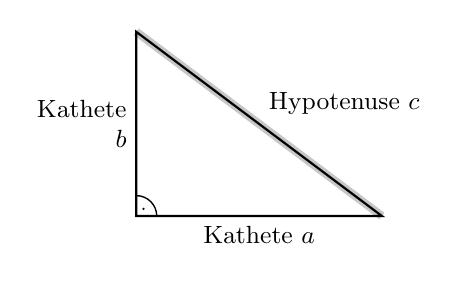
\begin{tikzpicture}[scale=0.52,font=\small]
\coordinate (C) at (0,0); \coordinate (B) at (6,0); \coordinate (A) at (0,4.5);
\draw[line width=3pt,black!22] (A) -- (B);
\draw[line width=0.8pt] (A) -- (B) -- (C) -- cycle;
\draw[line width=0.5pt] (0.5,0) arc (0:90:0.5); \fill (45:0.25) circle (0.9pt);
\node[below] at (3,0) {Kathete $a$}; \node[left,align=right] at (0,2.25) {Kathete\\$b$};
\node[above right] at (3,2.25) {Hypotenuse $c$};
\end{tikzpicture}
\end{minipage}
\end{tcolorbox}
\medskip\noindent\textbf{Typische Fehler – so nicht}\par\smallskip
\noindent\nr{$\times$}$c = a + b$ gerechnet. Richtig: erst quadrieren, addieren, dann die Wurzel.\par
\noindent\nr{$\times$}Eine Kathete als Hypotenuse genommen. Die Hypotenuse liegt dem rechten Winkel gegenüber.\par
\noindent\nr{$\times$}Wurzel vergessen: $c^2$ ist noch nicht $c$.\par
\noindent\nr{$\times$}Zwischendurch gerundet. Erst ganz am Ende runden.\par
\noindent\nr{$\times$}cm und m gemischt. Vorher beide Längen in dieselbe Einheit bringen.\par
\clearpage\label{s:A}\noindent\colorbox{black!12}{\makebox[10mm]{\Large\bfseries\strut A}}\hspace{3mm}{\Large\bfseries Hypotenuse finden und berechnen}\par\smallskip
\noindent Im rechtwinkligen Dreieck liegt dem rechten Winkel die längste Seite gegenüber: die \textbf{Hypotenuse}. Die beiden anderen Seiten heißen \textbf{Katheten}. Such immer zuerst den rechten Winkel – egal, wie das Dreieck liegt und wie die Seiten heißen.\par\medskip
\noindent\textbf{Formel}\par\nopagebreak\noindent\hspace*{4mm}\begin{minipage}{\dimexpr\linewidth-4mm\relax}$c^2 = a^2 + b^2$ \qquad also \qquad $c = \sqrt{a^2 + b^2}$ \qquad {\small ($c$ Hypotenuse, $a$ und $b$ Katheten)}\end{minipage}\par\medskip
\noindent\textbf{Beispiel}\quad Die Katheten sind 6\,cm und 8\,cm lang. Wie lang ist die Hypotenuse $c$?\par\smallskip
\noindent\begin{minipage}[t]{0.6\linewidth}\vspace{0pt}\par\noindent\hangindent6mm\hangafter1\makebox[6mm][l]{\textbf{1}}Rechter Winkel unten links. Gegenüber liegt $c$: die Hypotenuse.\par\smallskip\par\noindent\hangindent6mm\hangafter1\makebox[6mm][l]{\textbf{2}}$c^2 = 6^2 + 8^2 = 36 + 64 = 100$\par\smallskip\par\noindent\hangindent6mm\hangafter1\makebox[6mm][l]{\textbf{3}}$c = \sqrt{100} = 10$\par\smallskip\par\noindent\hangindent6mm\hangafter1\makebox[6mm][l]{\textbf{4}}Die Hypotenuse ist 10\,cm lang.\par\smallskip\end{minipage}\hfill
\begin{minipage}[t]{0.37\linewidth}\vspace{0pt}\centering 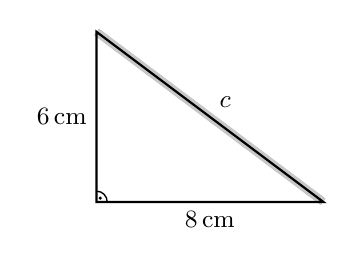
\begin{tikzpicture}[scale=0.36,font=\small]\coordinate (C) at (0,0); \coordinate (B) at (8,0); \coordinate (A) at (0,6);\draw[line width=3pt,black!22] (A) -- (B);\draw[line width=0.8pt] (A) -- (B) -- (C) -- cycle;\draw[line width=0.5pt] let \p1=($(B)-(C)$), \p2=($(A)-(C)$), \n1={atan2(\y1,\x1)}, \n2={atan2(\y2,\x2)}, \n3={ifthenelse(mod(\n2-\n1+360,360)<180,\n1,\n2)} in ($(C)+(\n3:0.38)$) arc (\n3:\n3+90:0.38) ($(C)+(\n3+45:0.19)$) circle (0.8pt);\node[below] at (4,0) {8\,cm}; \node[left] at (0,3) {6\,cm};\node[above right] at (4,3) {$c$};\end{tikzpicture}\end{minipage}\par\medskip
\noindent\textbf{Aufgaben}\hspace{1em}{\small\color{mbgrau}Rechne unten im Karo. Vergleiche jede Aufgabe gleich mit dem Lösungsheft.}\par\smallskip
\aufgg{\hangindent7mm\hangafter1\nr{1.}Das Dreieck liegt anders. Wo ist der rechte Winkel? Berechne die Hypotenuse $x$.}{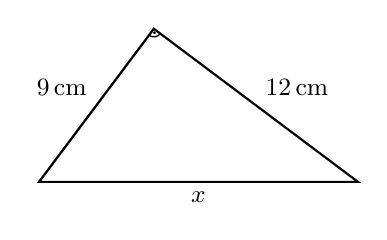
\begin{tikzpicture}[scale=0.27,font=\small]\coordinate (P) at (0,0); \coordinate (Q) at (15,0); \coordinate (R) at (5.4,7.2);\draw[line width=0.8pt] (P) -- (Q) -- (R) -- cycle;\draw[line width=0.5pt] let \p1=($(P)-(R)$), \p2=($(Q)-(R)$), \n1={atan2(\y1,\x1)}, \n2={atan2(\y2,\x2)}, \n3={ifthenelse(mod(\n2-\n1+360,360)<180,\n1,\n2)} in ($(R)+(\n3:0.38)$) arc (\n3:\n3+90:0.38) ($(R)+(\n3+45:0.19)$) circle (0.8pt);\node[above left] at (2.7,3.6) {9\,cm}; \node[above right] at (10.2,3.6) {12\,cm};\node[below] at (7.5,0) {$x$};\end{tikzpicture}}{}{}
\medskip
\aufgg{\hangindent7mm\hangafter1\nr{2.}Die Seiten heißen hier $r$, $s$ und $t$. (a) Schreib die Gleichung des Satzes für dieses Dreieck auf. (b) $r = 8$\,cm, $s = 15$\,cm. Berechne $t$.}{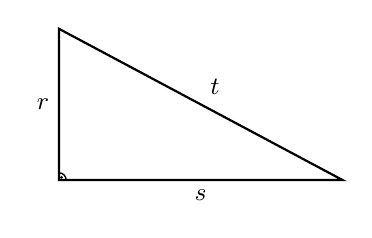
\begin{tikzpicture}[scale=0.24,font=\small]\coordinate (C) at (0,0); \coordinate (B) at (15,0); \coordinate (A) at (0,8);\draw[line width=0.8pt] (A) -- (B) -- (C) -- cycle;\draw[line width=0.5pt] let \p1=($(B)-(C)$), \p2=($(A)-(C)$), \n1={atan2(\y1,\x1)}, \n2={atan2(\y2,\x2)}, \n3={ifthenelse(mod(\n2-\n1+360,360)<180,\n1,\n2)} in ($(C)+(\n3:0.38)$) arc (\n3:\n3+90:0.38) ($(C)+(\n3+45:0.19)$) circle (0.8pt);\node[below] at (7.5,0) {$s$}; \node[left] at (0,4) {$r$};\node[above right] at (7.5,4) {$t$};\end{tikzpicture}}{}{}
\medskip
\aufgg{\hangindent7mm\hangafter1\nr{3.}Welche Gleichung passt zu diesem Dreieck? Kreuze an.\par\smallskip\leftskip7mm \kreuz{$u = v + w$}\ \kreuz{$u = \sqrt{v^2 - w^2}$}\par\kreuz{$u = v^2 + w^2$}\ \kreuz{$u = \sqrt{v^2 + w^2}$}}{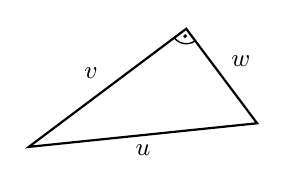
\begin{tikzpicture}[scale=0.5,font=\small]\coordinate (X) at (0,0); \coordinate (Y) at (4,3); \coordinate (Z) at (5.8,0.6);\draw[line width=0.8pt] (X) -- (Y) -- (Z) -- cycle;\draw[line width=0.5pt] let \p1=($(X)-(Y)$), \p2=($(Z)-(Y)$), \n1={atan2(\y1,\x1)}, \n2={atan2(\y2,\x2)}, \n3={ifthenelse(mod(\n2-\n1+360,360)<180,\n1,\n2)} in ($(Y)+(\n3:0.38)$) arc (\n3:\n3+90:0.38) ($(Y)+(\n3+45:0.19)$) circle (0.8pt);\node[above left] at (2,1.5) {$v$}; \node[above right] at (4.9,1.8) {$w$};\node[below] at (2.9,0.3) {$u$};\end{tikzpicture}}{}{}
\medskip
\aufgg{\hangindent7mm\hangafter1\nr{4.}Ein Schrank ist 240\,cm hoch und 70\,cm tief. Er wird liegend zusammengebaut und dann aufgerichtet; dabei kippt er über eine untere Kante. Das Zimmer ist 245\,cm hoch. Geht das? Begründe mit einer Rechnung. Tipp: Welche Strecke der Seitenwand ist am längsten?}{\begin{tikzpicture}[scale=0.62,font=\small]\draw[mbgrau] (-0.3,0) -- (7.4,0); \draw[mbgrau,dashed] (-0.3,4.6) -- (7.4,4.6);\node[above right,font=\scriptsize,mbgrau] at (-0.3,4.6) {Decke: 245\,cm hoch};\node[font=\scriptsize,mbgrau] at (2,-0.9) {nicht maßstabsgerecht};\draw[line width=0.8pt] (0,0) rectangle (4,1.17);\node[below] at (2,0) {240\,cm}; \node[right] at (4,0.58) {70\,cm};\draw[line width=0.8pt] (6,0) rectangle (7.17,4);\draw[->,mbgrau] (3.2,1.5) to[bend left=35] (5.8,3.0);\node[font=\scriptsize,mbgrau] at (3.4,2.9) {aufrichten};\end{tikzpicture}}{}{{\scriptsize\color{mbgrau}Ziel\hspace{2mm}}}
\medskip
\par\vspace{3mm}\newlength{\kr}\setlength{\kr}{\dimexpr\pagegoal-\pagetotal-10mm\relax}%
\ifdim\kr>12mm\noindent{\scriptsize\color{mbgrau}Platz zum Rechnen}\par\nointerlineskip\vspace{1mm}\noindent

\begin{tikzpicture}\clip (0,0) rectangle ({\linewidth-0.5mm},\kr);\draw[black!16,line width=0.3pt,step=5mm] (0,0) grid (\linewidth,\kr);\end{tikzpicture}\fi\par
\clearpage\label{s:B}\noindent\colorbox{black!12}{\makebox[10mm]{\Large\bfseries\strut B}}\hspace{3mm}{\Large\bfseries Wenn die Wurzel nicht aufgeht}\par\smallskip
\noindent Meist kommt keine glatte Zahl heraus. Dann schreibst du $c^2$ als Zwischenergebnis auf, ziehst die Wurzel mit dem Taschenrechner und rundest erst ganz am Ende.\par\medskip
\noindent\textbf{Formel}\par\nopagebreak\noindent\hspace*{4mm}\begin{minipage}{\dimexpr\linewidth-4mm\relax}$c^2 = a^2 + b^2$ \ \ $\to$ \ \ Wurzel ziehen: $c = \sqrt{c^2}$ \ \ $\to$ \ \ runden \ \ $\to$ \ \ Einheit\par {\small Vorher beide Längen in dieselbe Einheit bringen (1\,m = 100\,cm).}\end{minipage}\par\medskip
\noindent\textbf{Beispiel}\quad Die Katheten sind 7\,cm und 4\,cm lang. Berechne $c$ auf eine Stelle nach dem Komma.\par\smallskip
\noindent\begin{minipage}[t]{0.6\linewidth}\vspace{0pt}\par\noindent\hangindent6mm\hangafter1\makebox[6mm][l]{\textbf{1}}$c^2 = 7^2 + 4^2 = 49 + 16 = 65$\quad (Zwischenergebnis, nicht runden)\par\smallskip\par\noindent\hangindent6mm\hangafter1\makebox[6mm][l]{\textbf{2}}$c = \sqrt{65} \approx 8{,}062\ldots$\quad (Taschenrechner)\par\smallskip\par\noindent\hangindent6mm\hangafter1\makebox[6mm][l]{\textbf{3}}Runden auf eine Stelle: Danach kommt eine 6, also aufrunden.\par\smallskip\par\noindent\hangindent6mm\hangafter1\makebox[6mm][l]{\textbf{4}}$c \approx 8{,}1$\,cm\par\smallskip\end{minipage}\hfill
\begin{minipage}[t]{0.37\linewidth}\vspace{0pt}\centering 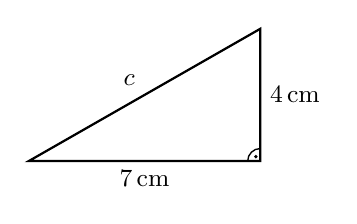
\begin{tikzpicture}[scale=0.42,font=\small]\coordinate (A) at (0,0); \coordinate (C) at (7,0); \coordinate (B) at (7,4);\draw[line width=0.8pt] (A) -- (C) -- (B) -- cycle;\draw[line width=0.5pt] let \p1=($(A)-(C)$), \p2=($(B)-(C)$), \n1={atan2(\y1,\x1)}, \n2={atan2(\y2,\x2)}, \n3={ifthenelse(mod(\n2-\n1+360,360)<180,\n1,\n2)} in ($(C)+(\n3:0.38)$) arc (\n3:\n3+90:0.38) ($(C)+(\n3+45:0.19)$) circle (0.8pt);\node[below] at (3.5,0) {7\,cm}; \node[right] at (7,2) {4\,cm};\node[above left] at (3.5,2) {$c$};\end{tikzpicture}\end{minipage}\par\medskip
\noindent\textbf{Aufgaben}\hspace{1em}{\small\color{mbgrau}Rechne unten im Karo. Vergleiche jede Aufgabe gleich mit dem Lösungsheft.}\par\smallskip
\aufg{\hangindent7mm\hangafter1\nr{1.}Ein rechtwinkliges Dreieck hat die Katheten 5\,cm und 9\,cm. Berechne die Hypotenuse. Runde auf eine Stelle nach dem Komma.}{}{}
\medskip
\aufg{\hangindent7mm\hangafter1\nr{2.}Die Katheten sind 2,5\,m und 4,2\,m lang. Berechne die Hypotenuse auf eine Stelle nach dem Komma.}{}{}
\medskip
\aufg{\hangindent7mm\hangafter1\nr{3.}Die Katheten sind 1,2\,m und 50\,cm lang. Mach zuerst beide Einheiten gleich. Wie lang ist die Hypotenuse?}{}{}
\medskip
\aufgg{\hangindent7mm\hangafter1\nr{4.}Der Bildschirm eines Handys ist 6,5\,cm breit und 14\,cm hoch. Wie lang ist seine Diagonale $d$? Runde auf eine Stelle nach dem Komma.}{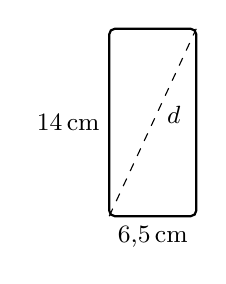
\begin{tikzpicture}[scale=0.17,font=\small]\draw[line width=0.8pt,rounded corners=2pt] (0,0) rectangle (6.5,14);\draw[dashed] (0,0) -- (6.5,14); \node[right] at (3.6,7.6) {$d$};\node[below] at (3.25,0) {6,5\,cm}; \node[left] at (0,7) {14\,cm};\end{tikzpicture}}{}{}
\medskip
\aufg{\hangindent7mm\hangafter1\nr{5.}Ein rechteckiger Park ist 160\,m lang und 70\,m breit. Lena will von einer Ecke zur gegenüberliegenden Ecke. Bisher ging sie außen am Rand entlang. Jetzt gibt es einen geraden Weg quer durch den Park. Wie viele Meter spart sie?}{}{{\scriptsize\color{mbgrau}Ziel\hspace{2mm}}}
\medskip
\par\vspace{3mm}\setlength{\kr}{\dimexpr\pagegoal-\pagetotal-10mm\relax}%
\ifdim\kr>12mm\noindent{\scriptsize\color{mbgrau}Platz zum Rechnen}\par\nointerlineskip\vspace{1mm}\noindent

\begin{tikzpicture}\clip (0,0) rectangle ({\linewidth-0.5mm},\kr);\draw[black!16,line width=0.3pt,step=5mm] (0,0) grid (\linewidth,\kr);\end{tikzpicture}\fi\par
\clearpage\label{s:C}\noindent\colorbox{black!12}{\makebox[10mm]{\Large\bfseries\strut C}}\hspace{3mm}{\Large\bfseries Sachaufgaben: Leiter, Rampe, Gelände}\par\smallskip
\noindent In Sachaufgaben steckt das Dreieck in der Wirklichkeit. Frag dich: Wo ist der rechte Winkel? Was liegt ihm gegenüber? Das ist die Hypotenuse.\par\medskip
\noindent\textbf{Formel}\par\nopagebreak\noindent\hspace*{4mm}\begin{minipage}{\dimexpr\linewidth-4mm\relax}rechter Winkel finden \ $\to$ \ Hypotenuse = gesuchte Strecke \ $\to$ \ $c^2 = a^2 + b^2$ \ $\to$ \ $c$ \ $\to$ \ Antwortsatz\par {\small Kommt noch etwas dazu (Knoten, Überstand): erst dazuzählen, dann runden – nicht zwischendurch.}\end{minipage}\par\medskip
\noindent\textbf{Beispiel}\quad Eine Leiter lehnt an einer Wand. Ihr Fuß steht 1,2\,m von der Wand weg, oben reicht sie 3,5\,m hoch. Wie lang ist die Leiter?\par\smallskip
\noindent\begin{minipage}[t]{0.6\linewidth}\vspace{0pt}\par\noindent\hangindent6mm\hangafter1\makebox[6mm][l]{\textbf{1}}Der rechte Winkel ist zwischen Wand und Boden.\par\smallskip\par\noindent\hangindent6mm\hangafter1\makebox[6mm][l]{\textbf{2}}Gegenüber liegt die Leiter: Sie ist die Hypotenuse $c$.\par\smallskip\par\noindent\hangindent6mm\hangafter1\makebox[6mm][l]{\textbf{3}}$c^2 = 1{,}2^2 + 3{,}5^2 = 1{,}44 + 12{,}25 = 13{,}69$\par\smallskip\par\noindent\hangindent6mm\hangafter1\makebox[6mm][l]{\textbf{4}}$c = \sqrt{13{,}69} = 3{,}7$\par\smallskip\par\noindent\hangindent6mm\hangafter1\makebox[6mm][l]{\textbf{5}}Antwort: Die Leiter ist 3,7\,m lang.\par\smallskip\end{minipage}\hfill
\begin{minipage}[t]{0.37\linewidth}\vspace{0pt}\centering \begin{tikzpicture}[scale=0.62,font=\small]\fill[black!12] (-0.35,0) rectangle (0,4.1); \draw[line width=0.8pt] (0,0) -- (0,4.1);\draw[line width=0.8pt] (-0.35,0) -- (2.4,0);\draw[line width=1.6pt] (1.2,0) -- (0,3.5); \node[right] at (0.65,2.0) {$c$};\draw[line width=0.5pt] let \p1=($(1,0)-(0,0)$), \p2=($(0,1)-(0,0)$), \n1={atan2(\y1,\x1)}, \n2={atan2(\y2,\x2)}, \n3={ifthenelse(mod(\n2-\n1+360,360)<180,\n1,\n2)} in ($(0,0)+(\n3:0.38)$) arc (\n3:\n3+90:0.38) ($(0,0)+(\n3+45:0.19)$) circle (0.8pt);\draw[|<->|,mbgrau] (0,-0.35) -- (1.2,-0.35); \node[below] at (0.6,-0.35) {1,2\,m};\draw[|<->|,mbgrau] (-0.6,0) -- (-0.6,3.5); \node[left] at (-0.6,1.75) {3,5\,m};\end{tikzpicture}\end{minipage}\par\medskip
\noindent\textbf{Aufgaben}\hspace{1em}{\small\color{mbgrau}Rechne unten im Karo. Vergleiche jede Aufgabe gleich mit dem Lösungsheft.}\par\smallskip
\aufgg{\hangindent7mm\hangafter1\nr{1.}Eine Rampe führt auf eine Stufe. Sie ist waagerecht gemessen 240\,cm lang, die Stufe ist 18\,cm hoch. Wie lang ist die schräge Rampe? Runde auf eine Stelle nach dem Komma.}{\begin{tikzpicture}[scale=0.62,font=\small]\draw[line width=0.8pt] (0,0) -- (5,0) -- (5,0.7) -- cycle;\fill[black!12] (5,0) rectangle (5.8,0.7); \draw (5,0.7) -- (5.8,0.7) -- (5.8,0);\draw[line width=0.5pt] let \p1=($(0,0)-(5,0)$), \p2=($(5,0.7)-(5,0)$), \n1={atan2(\y1,\x1)}, \n2={atan2(\y2,\x2)}, \n3={ifthenelse(mod(\n2-\n1+360,360)<180,\n1,\n2)} in ($(5,0)+(\n3:0.38)$) arc (\n3:\n3+90:0.38) ($(5,0)+(\n3+45:0.19)$) circle (0.8pt);\node[below] at (2.5,0) {240\,cm}; \node[right,font=\scriptsize] at (5.8,0.35) {18\,cm};\node[above left] at (2.5,0.35) {$x$};\node[font=\scriptsize,mbgrau] at (2.6,-0.9) {nicht maßstabsgerecht};\end{tikzpicture}}{}{}
\medskip
\aufgg{\hangindent7mm\hangafter1\nr{2.}Zwischen $A$ und $B$ liegt ein Teich. Man misst über $C$ (rechter Winkel bei $C$): $\overline{CA} = 34$\,m, $\overline{CB} = 12$\,m. Wie weit ist $A$ von $B$ entfernt? Gib auch das Zwischenergebnis $\overline{AB}^{\,2}$ an. Achtung: Welche Seite ist die längste?}{\begin{tikzpicture}[scale=0.62,font=\small]\coordinate (C) at (0,0); \coordinate (A) at (0,3.4); \coordinate (B) at (2.4,0);\fill[black!10,rotate around={-54.8:(1.2,1.7)}] (1.2,1.7) ellipse (0.9 and 0.45);\draw[line width=0.8pt] (A) -- (C) -- (B); \draw[dashed] (A) -- (B);\draw[line width=0.5pt] let \p1=($(B)-(C)$), \p2=($(A)-(C)$), \n1={atan2(\y1,\x1)}, \n2={atan2(\y2,\x2)}, \n3={ifthenelse(mod(\n2-\n1+360,360)<180,\n1,\n2)} in ($(C)+(\n3:0.38)$) arc (\n3:\n3+90:0.38) ($(C)+(\n3+45:0.19)$) circle (0.8pt);\fill (A) circle (1.5pt) node[above] {$A$}; \fill (B) circle (1.5pt) node[right] {$B$};\fill (C) circle (1.5pt) node[below left] {$C$};\node[left] at (0,1.7) {34\,m}; \node[below] at (1.2,0) {12\,m};\node[font=\scriptsize,mbgrau] at (1.25,1.75) {Teich};\end{tikzpicture}}{}{}
\medskip
\aufgg{\hangindent7mm\hangafter1\nr{3.}Ein Fahnenmast wird mit einem Seil gesichert. Das Seil ist in 6\,m Höhe am Mast befestigt und 3\,m vom Mast entfernt im Boden. Für die zwei Knoten braucht man zusätzlich 0,5\,m Seil. Wie lang muss das Seil sein? Runde auf eine Stelle nach dem Komma.}{\begin{tikzpicture}[scale=0.33,font=\small]\draw[line width=0.8pt] (-0.6,0) -- (3.8,0); \draw[line width=1.6pt] (0,0) -- (0,8);\fill[black!25] (0,8) -- (1.6,7.5) -- (0,7) -- cycle;\draw[line width=0.8pt] (0,6) -- (3,0);\draw[line width=0.5pt] let \p1=($(1,0)-(0,0)$), \p2=($(0,1)-(0,0)$), \n1={atan2(\y1,\x1)}, \n2={atan2(\y2,\x2)}, \n3={ifthenelse(mod(\n2-\n1+360,360)<180,\n1,\n2)} in ($(0,0)+(\n3:0.38)$) arc (\n3:\n3+90:0.38) ($(0,0)+(\n3+45:0.19)$) circle (0.8pt);\node[right] at (1.6,3.2) {Seil};\draw[|<->|,mbgrau] (-1.1,0) -- (-1.1,6); \node[left] at (-1.1,3) {6\,m};\node[below] at (1.5,0) {3\,m};\end{tikzpicture}}{}{}
\medskip
\aufg{\hangindent7mm\hangafter1\nr{4.}Herr Kaya will an ein Fenster. Die Unterkante liegt 4,70\,m hoch. Seine Leiter ist 5\,m lang. Wegen eines Beetes muss der Fuß der Leiter 2\,m von der Hauswand entfernt stehen. Reicht die Leiter bis zur Unterkante? Wie lang müsste die Leiter mindestens sein? Wie viel fehlt? Rechne mit zwei Stellen nach dem Komma.}{}{{\scriptsize\color{mbgrau}Ziel\hspace{2mm}}}
\medskip
\par\vspace{3mm}\setlength{\kr}{\dimexpr\pagegoal-\pagetotal-10mm\relax}%
\ifdim\kr>12mm\noindent{\scriptsize\color{mbgrau}Platz zum Rechnen}\par\nointerlineskip\vspace{1mm}\noindent

\begin{tikzpicture}\clip (0,0) rectangle ({\linewidth-0.5mm},\kr);\draw[black!16,line width=0.3pt,step=5mm] (0,0) grid (\linewidth,\kr);\end{tikzpicture}\fi\par
\clearpage\label{s:T}\noindent\colorbox{black!12}{\makebox[10mm]{\Large\bfseries\strut T}}\hspace{3mm}{\Large\bfseries Probetest}\par\smallskip
\noindent Gemischt wie in der Prüfung, ohne Beispiel. Taschenrechner erlaubt. Etwa 20 Minuten.\par\medskip
\noindent\textbf{Aufgaben}\hspace{1em}{\small\color{mbgrau}Rechne unten im Karo. Vergleiche jede Aufgabe gleich mit dem Lösungsheft.}\par\smallskip
\aufg{\hangindent7mm\hangafter1\nr{1.}Welche Aussage ist der Satz des Pythagoras? Kreuze an.\par\smallskip\leftskip7mm \kreuzl{In einem rechtwinkligen Dreieck ist die Hypotenuse so lang wie die beiden Katheten zusammen.}\kreuzl{In einem rechtwinkligen Dreieck ist die Summe der Flächeninhalte der Kathetenquadrate gleich dem Flächeninhalt des Hypotenusenquadrats.}\kreuzl{In einem rechtwinkligen Dreieck liegt dem rechten Winkel eine Kathete gegenüber.}}{}{}
\medskip
\aufgg{\hangindent7mm\hangafter1\nr{2.}Welche Gleichung gilt für dieses Dreieck? Kreuze an.\par\smallskip\leftskip7mm \kreuz{$c^2 = a^2 + b^2$}\ \kreuz{$a^2 = b^2 + c^2$}\par\kreuz{$b^2 = a^2 + c^2$}\ \kreuz{$a = b + c$}}{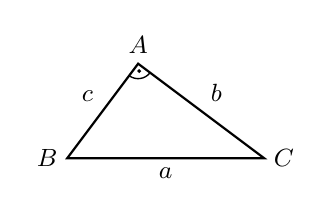
\begin{tikzpicture}[scale=0.5,font=\small]\coordinate (A) at (1.8,2.4); \coordinate (B) at (0,0); \coordinate (C) at (5,0);\draw[line width=0.8pt] (A) -- (B) -- (C) -- cycle;\draw[line width=0.5pt] let \p1=($(B)-(A)$), \p2=($(C)-(A)$), \n1={atan2(\y1,\x1)}, \n2={atan2(\y2,\x2)}, \n3={ifthenelse(mod(\n2-\n1+360,360)<180,\n1,\n2)} in ($(A)+(\n3:0.38)$) arc (\n3:\n3+90:0.38) ($(A)+(\n3+45:0.19)$) circle (0.8pt);\node[above] at (A) {$A$}; \node[left] at (B) {$B$}; \node[right] at (C) {$C$};\node[below] at (2.5,0) {$a$}; \node[above right] at (3.4,1.2) {$b$};\node[above left] at (0.9,1.2) {$c$};\end{tikzpicture}}{}{}
\medskip
\aufg{\hangindent7mm\hangafter1\nr{3.}Ein Fußballfeld ist 105\,m lang und 68\,m breit. Ein Spieler läuft auf gerader Linie von einer Eckfahne zur gegenüberliegenden. Wie lang ist sein Weg? Gib das Zwischenergebnis an und runde auf eine Stelle nach dem Komma.}{}{}
\medskip
\aufg{\hangindent7mm\hangafter1\nr{4.}Familie Berg zieht um. Eine Gardinenstange ist 2,60\,m lang. Der Boden des Laderaums im Transporter ist 2,20\,m lang und 1,30\,m breit. Kann die Stange flach auf dem Boden liegen? Begründe mit einer Rechnung.}{}{{\scriptsize\color{mbgrau}Ziel\hspace{2mm}}}
\medskip
\par\vspace{3mm}\setlength{\kr}{\dimexpr\pagegoal-\pagetotal-10mm\relax}%
\ifdim\kr>12mm\noindent{\scriptsize\color{mbgrau}Platz zum Rechnen}\par\nointerlineskip\vspace{1mm}\noindent

\begin{tikzpicture}\clip (0,0) rectangle ({\linewidth-0.5mm},\kr);\draw[black!16,line width=0.3pt,step=5mm] (0,0) grid (\linewidth,\kr);\end{tikzpicture}\fi\par
\end{document}
